\documentclass[11pt,a4paper,utf8]{article} 
\usepackage{fontspec}
\setmainfont{Times New Roman}    

\usepackage{abstract} 
\usepackage{amsmath}  
\usepackage{authblk}
\usepackage{array} 
\usepackage{booktabs} %绘制表格  
\usepackage{biblatex} 
\usepackage{caption2} %标题居中
\usepackage{color} 
\usepackage{colortbl}
\usepackage{ctex}
\usepackage{enumerate}  
\usepackage{float}
\usepackage{fontspec}
\usepackage{geometry} 
\usepackage{graphicx}  
\usepackage[hidelinks]{hyperref}
\usepackage{listings} 
\usepackage{longtable} 
\usepackage{multirow}
\usepackage{biblatex}
\usepackage{subfigure}
\usepackage{soul}
\usepackage{titlesec}  
\usepackage{fancyhdr} % 导入fancyhdr包



\geometry{a4paper, left=2.5cm, right=2.5cm, top=2.5cm, bottom=2.5cm}%设置页面尺寸
\lstset{
		numbers=left, %设置行号位置
		numberstyle=\tiny, %设置行号大小
		keywordstyle=\color{blue}, %设置关键字颜色
		commentstyle=\color[cmyk]{1, 0, 1, 0}, %设置注释颜色
		escapeinside=``, %逃逸字符(1左面的键), 用于显示中文
		breaklines, %自动折行
		extendedchars=false, %解决代码跨页时, 章节标题, 页眉等汉字不显示的问题
		xleftmargin=1em, xrightmargin=1em, aboveskip=1em, %设置边距
		tabsize=4, %设置tab空格数
		showspaces=false %不显示空格
}

\pagestyle{fancy}
% 页眉设置  
\fancyhead[L]{}
% \fancyhead[C]{网络舆情分析行业大数据相关调查报告}
% \fancyhead[R]{}
% 页脚设置
\fancyfoot[C]{\thepage} % 页码
\renewcommand{\headrulewidth}{2pt} % 分隔线宽度2磅
\renewcommand{\footrulewidth}{1pt}

   
\title{\HUGE{\textbf{网络舆情分析行业大数据相关调查报告}}}
\author[1]{王红阳}
\author[2]{夏睿} 
\author[3]{周浩然}
\author[4]{窦浩阳}

\affil[1]{天津大学智能与计算学部-3019244233}
\affil[2]{天津大学智能与计算学部-3019244105} 
\affil[3]{天津大学智能与计算学部-3019244229} 
\affil[4]{天津大学智能与计算学部-3019202235} 
\renewcommand*{\Affilfont}{\small\it} % 修改机构名称的字体与大小
% \date{} % 去掉日期


\begin{document}
\pagenumbering{Roman} %设置罗马数字页码

\begin{figure}[t]
\centering
	
\includegraphics[scale=0.6]{images/图标.png} 
\end{figure}


\maketitle % 显示标题
 
% \phantomsection\addcontentsline{toc}{section}{摘要}\tolerance=500
% \begin{abstract}
% \normalsize
% % 这里应该写个摘要
 
 
% \textbf{[Key Words]}:  网络舆情分析、海量数据、社交媒体、舆论管理、行业分析
% \end{abstract}


% \thispagestyle{empty} % 取消页脚

\newpage %分页
\pagenumbering{arabic} %设置数字页码

\thispagestyle{empty} % 取消页脚
% 目录
\renewcommand{\contentsname}{\centerline{ 目 \quad 录}}
\begin{center}
    \tableofcontents
\end{center}

\setcounter{page}{0}
\thispagestyle{empty} % 取消页脚
 
 
  
\newpage  
\section{网络舆情大数据的现状、面临挑战及意义} 

{\color{red}{以下部分由王红阳书写整理}}
\subsection{网络舆情大数据现状}
互联网+ 时代来临,随时随地发布新闻、了解咨询、关注国计民生以及发表个人观点和看法成为新常态。舆情的发生、发展、演化及传播等特点发生着翻天覆地的变化,与之相应的舆情监测、分析和决策方法日益成为关注的焦点$^{[1]}$。\\

与此同时,大数据给网络舆情带来了新的挑战:

\subsection{网络舆情大数据的挑战} 
\subsubsection{海量数据}
海量网络信息难以掌控,大量相关性、偶发性因素使舆情更加复杂多变,传统的舆情监测手段和方法难以奏效。

\subsubsection{信息选择性传播}
网上数据无限性和网民关注能力有限性之间的矛盾,加剧了社会舆论的“盲人摸象”效应。社会化媒体促进信息的开放和沟通的便捷,分众传播、个性化传播凸显,使偏激的观点更容易找到“同类”,从而加剧舆论偏激情绪。 

\subsubsection{舆论话语权分散}
大数据时代各类数据随手可得,越来越多的机构、个人通过数据挖掘和分析得出的各种结论迅速传播,有效管理舆情的难度越来越大$^{[2]}$。 \\


\begin{figure}[H]
\centering 
\subfigure 
{  
    \begin{minipage}[b]{.4\linewidth}
        \centering
        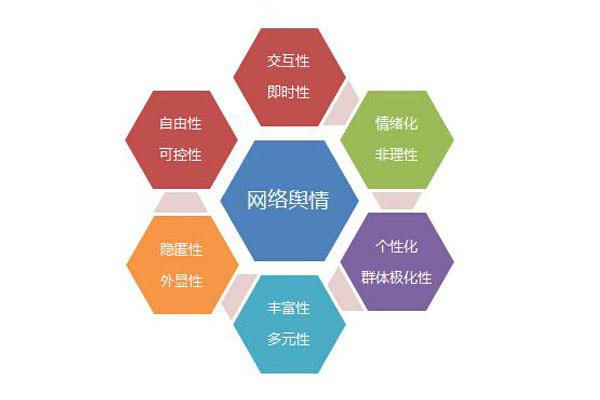
\includegraphics[scale=0.45]{images/六边形.png}
     \end{minipage}
}
\subfigure 
{  
    \begin{minipage}[b]{.4\linewidth}
        \centering
        
\includegraphics[scale=0.45]{images/词云图.png}
    \end{minipage}
     
}
\caption{网络舆情的关键词云及特性}
\end{figure}

另外,以新冠肺炎为例,突发公共事件网络舆情具有突发性、扩散性、匿名性和多元性的特点。大数据环境下,相关部门暴露出采集效率低、可靠性差、分析力度不足、分析能力欠缺的问题,导致在实际网络舆情分析应用过程中,不能及时发现事件隐藏信息,出现舆情判断失误$^{[3]}$。

\subsection{网络舆情大数据的新机遇及意义}


\begin{enumerate}
\item 拓展网络舆情治理领域。在“一切皆可量化”的大数据浪潮中,网络社会与现实社会日益融为一体,网络舆情管理不再局限于网上言论领域,必须全面掌握网络舆情运行规律及其与现实社会的相互影响,实现网上网下联动共治。 

\item 丰富网络舆情管理手段。运用大数据技术,可以从更宽领域、更长时段对网上舆论进行比对分析,更加准确地把握网民情绪特点,预判舆情发展趋势,提高舆情管理的效能。例如网络评论数据处理技术的应用,不仅能够提升数据分析、提取、整理和研究的效果,还能转变传统的数据处理形式,有效完成各项数据处理的任务$^{[4]}$ 。 

\item 对于突发事件舆情,应用大数据技术可以帮助相关部门对舆情信息进行及时采集和分析应对,最大限度降低突发事件所带来的不良社会影响,引导公众树立正确的舆论观,促进社会和谐发展。 

\end{enumerate}
  

\section{网络舆情大数据相关机构及其进展}

{\color{red}{以下部分由夏睿书写整理}} 

\subsection{网络舆情大数据相关体系}
当前,舆情大数据在企业中已有完整的应用体系,主要分为 4 个模块:
\begin{enumerate}
\item \textbf{网络舆情监测:}对网络数据进行针对性部署,实现境内境外,多语言,多载体,多纬度24小时的实时监控,及时获得各类数据
\item \textbf{网络舆情分析:} 对获取的数据信息进行分析,判断是否与客户相关,解析舆论信息情感,分析热点,寻找传播途径等,深度挖掘网络舆情的大数据中的有效情报
\item \textbf{网络舆情管理:} 制定舆情管理业务标准,做到舆情早监测,早发现,早处置,早导控。形成一套完整的舆情分类管理体系
\item \textbf{网络舆情应对:} 针对不同的舆情制定不同的应对策略,及时预警,控制舆论,争取舆论高度,形成意见领袖 
\end{enumerate}

\subsection{国内外舆情分析知名企业机构} 
国内外已经有许多大数据公司涉足舆情领域,如国内的中科点击、泰一指尚、谷尼、中国舆情网等;国外的 Cision、Reputation Defender、Nielsen等。 \\

这些大数据公司或对舆情数据提供整套的体系服务,或专门为其中某个环节提供服务,例如中科点击,Cision 都提供整套解决方案,Reputation Defender专门提供网络舆情应对的服务。
 

\begin{figure}[H]
\centering 
\subfigure 
{  
    \begin{minipage}[b]{.4\linewidth}
        \centering
        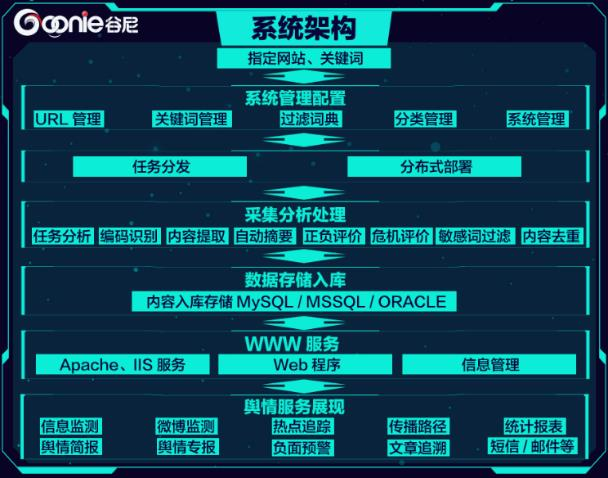
\includegraphics[scale=0.45]{images/谷尼.png}
     \end{minipage}
}
\subfigure 
{  
    \begin{minipage}[b]{.4\linewidth}
        \centering
        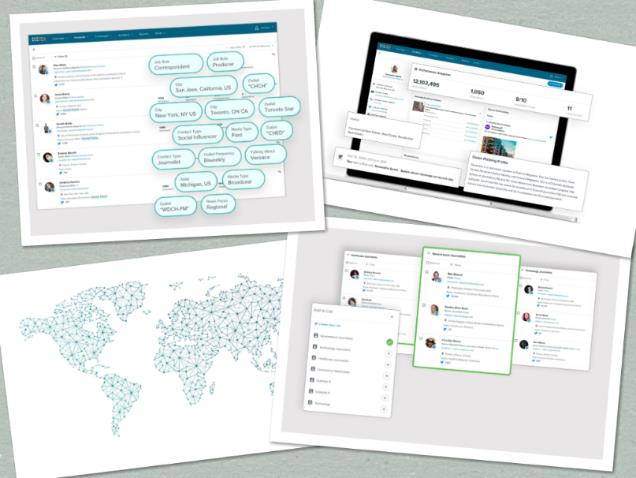
\includegraphics[scale=0.45]{images/cision.png} 
    \end{minipage}
}
\caption{国内公司谷尼的舆情处理体系(左)、Cision 的舆情管理关系网(右)}
\end{figure}


\subsubsection{Cision & Reputation Defender}
Cision 拥有最完整的全球在线新闻、博客、社交、印刷和广播频道集合,来源超过700万个,可以实时跟踪品牌情况。\\

在管理方面,Cision 拥有一个专业的数据库,它提供了140万名经过专业策划的记者、媒体、以及超过 10 亿的社会影响者的简介,可帮助客户直接与目标受众进行直接交流;根据舆情信息分析受众信息,对目标受众进行产品、广告的精准推送。 \\

合作企业包括 3M(美国明尼苏达矿务及制造业公司)、PBS(美国公共电视网)、Citrix(美国思杰云计算虚拟化公司)等。 \\

Reputation Defender专门负责舆情应对服务,可通过更改网页权重控制搜索结果,更改舆情推广产品;定期扫描网络信息并隐藏或删除客户指定的隐私信息;鼓励用户对产品进行评价,审核控制评价内容,控制舆论创建企业形象。\\

\subsubsection{军犬舆情监测系统}
中科点击推出的“ 军犬系列”为其舆论大数据监测的主要平台:\\

“军犬舆情监测系统”采用Hadoop数据信息分析平台对全网信息进行实时监控,最早推出了多语言舆情监控,集成了多家网络信息载体平台,对非结构化信息进行结构抽取及数据存储,记录舆情传播途径,及时获取各方面信息。\\

“军犬网评”提供了网评任务发布平台,这对应了舆情体系中的舆情应对,根据前面分析出的舆情核心及舆情情感等信息发布相应任务,包括浏览、发帖、点赞、转发等,对舆情进行控制或引导,占领舆情高地,影响舆情热度、排序、观点等属性,为客户提供最有利的舆情氛围。\\

目前合作对象包括各省市国安厅公安厅,国防科技大学、北科院等科研院校,各大通信运营商、银行、汽车等企业。\\


% \begin{figure}[H]
%     \centering
%     
\includegraphics[width=0.6\textwidth]{images/军犬.png}  
%     \caption{军犬网评应对舆情} 
% \end{figure}  


\subsection{行业未来展望}
通过对舆情领域公司的调研可以发现,所有相关企业本质上仍是大数据企业,只有对舆情大数据进行有效收集、分析、处理、应对、有成熟的把控大数据的技术,才能真正地为客户提供良好的舆情相关的服务。 \\ 

在未来,这些公司将继续围绕舆情体系的一个或多个环节进行产品更新,例如在分析环节通过更高效的挖掘获取更多维度的信息,在管理环节构造更加有效的舆情应对关系网,为舆情提供更多元的解决方案。 \\

\section{网络舆情分析相关前沿论文及研究方法}

{\color{red}{以下部分由周浩然书写整理}} \\
网络舆情大数据相关研究对提升政府科学管理水平和社会治理能力有重要意义。近年来,基于大数据的多种算法,在网络舆情分析领域中起到了重要作用。\\

\subsection{主题模型}

LDA(隐含狄利克雷分配)主题模型是网络舆情大数据分析中常用的建模方法。\\

LDA 主题模型是一种基于贝叶斯概率的由词项、主题、文档三层结构组成的文本分类模型。LDA主题模型通过无监督的方式学习文本中隐含的主题信息,利用文本中词项的共现特征来发现文本的主体结构。 \\ 

LDA 主题模型中,一篇文档的生成过程如下: 
\begin{enumerate}
\item 从给定的狄利克雷分布中取样生成文档和主题分布
\item 从主题的多项式分布中取样生成文档中词汇的主题
\item 从狄利克雷分布中取样生成主题,及对应词语分布
\item 从词语的多项式分布中采样生成最终的词汇集合
\end{enumerate}
 

相关研究和实践$^{[5][6]}$表明,微博评论、贴吧回帖等大多数网络舆情文本数据由于长度较短,传统分类模型无法充分发掘短文本的序列信息,而LDA主题模型可以充分挖掘短文本的主题信息,提高分类准确度。

\subsection{情感倾向分析模型}
LSTM(长短期记忆神经网络)模型可以有效地用于分析用户情感倾向,常常需要与词向量计算工具配合使用。word2vec 是谷歌开源的词向量计算模型,该模型可以根据给定的语料库进行学习,而后快速有效的将一个词语表达为向量形式。 \\

实际研究过程$^{[7]}$ 中,基于LSTM的网络舆情和用户情感倾向分析流程一般为以下三个步骤:
\begin{enumerate}
\item 通过爬虫爬取微博、贴吧等话题数据;
\item 利用 word2Vec 模型训练词向量;
\item 基于预训练的 LSTM 模型实现舆情情感分类。
\end{enumerate} 

分析表明,基于深度学习的舆情分析模型相较于传统方法可以挖掘出数据更深层的关系和内涵,具有一定的优越性

\subsection{舆论场建模}
近年来,网络舆情分析和治理领域的相关学者提出了舆论场的概念,创造性的将场论引入舆情研究中,从而提出了众多新颖的思想和方法。\\

王玉珠$^{[8]}$ 基于对众多社会事件的舆情观察提出了微信舆论场的概念,并对微信舆论场的特点进行了研究概括:网络封闭复杂、以紧密型人际关系网络为主、间接推动舆情。通过引入微信舆论场的概念,该文作者对后续微信舆情的研究方向提出了建议:识别微信舆论领袖、分析微信舆情与事件的关联并进行趋势预测。\\

基于舆论场的思想,相关学者$^{[9]}$通过BI-LSTM-CRF、K-Means、TF-IDF等机器学习、主题提取方法的结合,实现了对网络舆情的演化进行了多角度的分析。\\

联系目前所学知识,基于舆论场的思想,对于舆论场内领袖可以通过PageRank、图模型等算法进行分析,对于舆情趋势可以采用 RNN、LSTM等时序模型进行分析预测。并结合Spark等大数据分析平台,对舆论大数据进行实时流式分析,以满足舆论分析的时效性需求。\\

\section{社交媒体:Web2.0 时代舆情大数据来源}

{\color{red}{以下部分由窦浩阳书写整理}} 
\subsection{基于社交媒体的舆情大数据分析意义}

随着社交媒体平台用户量的不断激增与功能的逐步拓展,社交媒体已经渐趋成为一种强大的文化、政治力量,开始有能力改变一些国内甚至全球性事件的走向$^{[10]}$。美国是社交媒体的诞生地,长期以来,美国政府都将社交媒体作为重要的执政工具,但当社交媒体全方位主导2016年美国总统竞选,并在特朗普“推特执政”格局下进一步加剧美国的政治极化与社会撕裂时,社交媒体已从美国政府管理与推广民主的得力工具沦为暴露自身民主乱象的显示器,社交媒体时代美国网络舆情治理困境尽显。\\

习近平总书记指出:“网络已是当前意识形态斗争的最前沿。掌控网络意识形态主导权,就是守护国家的主权和政权”$^{[11]}$。随着互联网的媒介属性越来越凸显,加之在这个过程中,传播快、影响大、覆盖广、社会动员能力强的“两微一抖”等社交媒体用户也呈快速增长趋势,网络舆论与官方舆论“两个舆论场”并存、对垒的格局渐趋形成。如何吸取以美国为代表的西方主要大国在网络舆情治理过程中积累的经验教训,确保网络信息传播秩序和国家安全、社会稳定,已经成为摆在我们面前的突出现实问题。\\
 
% \subsection{主要社交应用使用情况(截至 2020 年 1 月)} 
% \begin{table}[H]   
% \centering
% \newcommand{\tabincell}[2]{\begin{tabular}{@{}#1@{}}#2\end{tabular}}  %导言区
% \caption{主要社交网站使用情况(截至 2020 年 1 月)$^{[12]}$}  
% \begin{tabular}{|c|c|c|c|}   
% \hline   
% \textbf{社交网站 } & \textbf{创立时间} & \textbf{活跃用户量} & \textbf{功能特征}  \\ 
% \hline 
% \tabincell{c}{ \\  }
% Facebook & 2004年 & & \tabincell{c}{ 全球第一大社交网站,允许用户创建自己的个人资料,  \\  分享照片和视频,并与其他用户沟通 } \\  
% \hline 
% YouTube & 2005 年 & & \tabincell{c}{在线视频服务网站,为用户提供视频上传、分发、 \\ 展示、浏览服务} \\ 
% \hline 
% WhatsApp & 2009 年 & &  \tabincell{c}{智能手机即时通讯应用程序,支持发送和接收文字、\\ 图片、音频和视频信息} \\
% \hline 
% \tabincell{c}{WeChat \\ (微信) }& 2011 年 & & \tabincell{c}{智能手机即时通讯应用程序,支持发送和接收文字、\\ 图片、音频和视频信息}  \\
% \hline 
% Instagram & 2010 年 & & \tabincell{c}{图片分享移动应用程序,融入社交化元素,包括\\ 好友关系建立、回复、分享及收藏等} \\
% \hline 
% \tabincell{c}{Tik Tok \\ (抖音) }& 2016 年 & & \tabincell{c}{短视频社交应用程序,用户可以自主选择歌曲、\\拍摄音乐短视频,支持视频拍摄快慢、\\ 视频编辑、特效等} \\
% \hline 
% \tabincell{c}{Sina Weibo \\ (新浪微博)} & 2009 年 & & \tabincell{c}{ 社交网络及微博服务网站,用户可通过 \\  网页、手机移动程序等发布动态,\\ 并可上传图片和视频或进行视频直播} \\
% \hline 
% Twitter  & 2006 年 & &  \tabincell{c}{社交网络及微博服务网站,作为即时通讯的变种, \\ 向用户推送其感兴趣的实时更新, \\ 并通过多个视角使事件得以实时呈现}  \\
% \hline
% \end{tabular}    
% \end{table}     

\subsection{社交APP大数据获取方式(以 Twitter 为例)}
在随着数字化媒体浪潮的到来,第三方开发的网站应用已经成为社交网络必不可少的一部分。除了开发人员进行基础爬虫之外,社交网站为了自身的发展,往往选择向外界开放部分资源,以方便第三方发展基于该社交网站的产品,进而更好吸引使用者使用。\\

以 Twitter 为例$^{[12]}$ ,Twitter 通过 API 的方式开放一些应用接口,目前仅支持 HTTP Basic Authentication 验证机制。当使用 HTTP Basic Authentication时,需使用在Twitter注册的“用户名”作为 Session 或 Cookie 的“用户名”部分的内容。\\

Twitter API 可以满足多种数据爬取需求,包括:用 Search API 找到历史推文;用实时streaming API 过滤功能得到想要的推文;基于用户在其公开个人资料中提供的“主页”位置,这是一个自由格式的字符字段,可能包含也可能不包含可以进行地理参考的元数据。
 

 
\section{网络舆情大数据待解决问题}
{\color{red}{以下部分由王红阳书写整理}} 

\subsection{舆情治理体系不完备问题}
目前,我国互联网法律法规并不能完全解决网络舆情管理问题,网络舆情组织形式日益专业化,恶意炒作和造谣诋毁事件时有发生。我国政府部门着眼于加强网络舆情监测,需要创新大数据舆情收集分析技术,完善大数据信息管理机制,进一步完善舆情引导机制$^{[13]}$ 。

\subsection{情绪衡量偏误问题}
舆情中包含了情绪,判定民众在某一事件的情绪的正负性需要对文本进行分析。然而,现实世界中情绪的高度复杂性和语言的语义模糊性对情绪的区分造成了严重的阻碍,比如对反讽类型的评论进行情绪提取往往提取出相反的情绪结果。

\subsection{样本截断问题}
由于网络平台使用存在一定门槛,从而天然排除了不能使用网络媒体或经济地位较低无法负担网络媒体者的意见。而且,网络上的意见表达只是网民意见表达的一部分行为,大量舆情行为发生在线下,是无法观测到的。在这个意义下,大数据搜集的是截断数据,会一定程度上影响舆情监测的稳健性。

\begin{figure}[H]
    \centering
    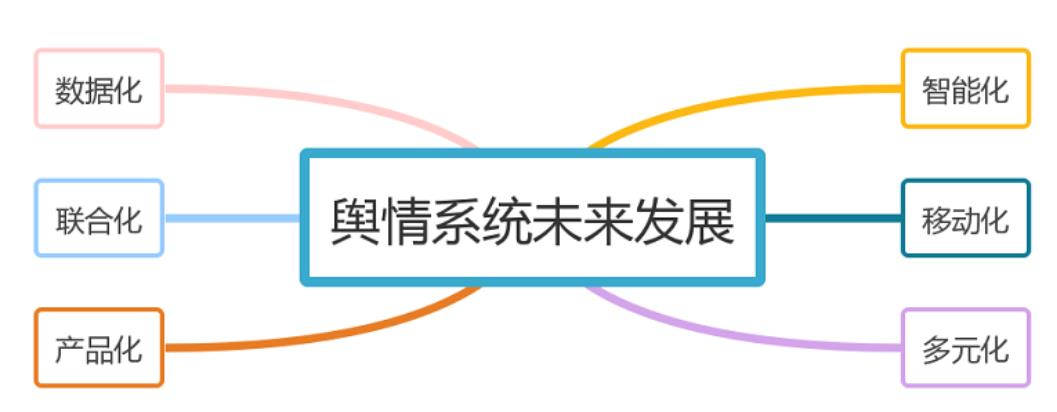
\includegraphics[width=0.7\textwidth]{images/舆情.png}  
    \caption{舆情系统发展趋势} 
\end{figure}  

\section{网络舆情大数据未来发展方向}

{\color{red}{以下部分由王红阳书写整理}} 

\subsection{多元产业链}
舆情监测是串联企业业务重要的一环。舆情监测公司只有掌握核心技术才能存活,而大多数公司要向多元化的服务和开拓新的需求来谋求发展。

\subsection{移动化和智能化}
目前市场上还没有完全取代人工的舆情监测系统,时效性是亟待解决的问题,所以智能化是未来行业发展的一个标志性方向。移动互联网时代,人们的工作重心逐渐从PC端转移到移动应用,所以舆情监测企业未来重心将转移至移动端。

\subsection{联合化和产品化}
高校和新闻媒体为舆情分析机构提供数据来源和用户,机构为高校和新闻媒体提供分析结果和预警,实现双赢。整合资源,开发新产品,构建完整的网络舆情监测产业链,提供快、准、全的舆情。
 
\newpage %分页  
\addcontentsline{toc}{section}{参考文献} 
\begin{thebibliography}{99}  
\small
\bibitem{ref1}Bruce.大数据的舆情分析与决策方法[EB/OL].https://zhuanlan.zhihu.com/p/57752782
\bibitem{ref2}中正舆情.大数据时代的网络舆情管理[EB/OL].https://zhuanlan.zhihu.com/p/57752782
\bibitem{ref3}杜乐谊.大数据在突发事件网络舆情分析中的应用[J].中国信息化,2020(11):54-55.
\bibitem{ref4}杨康.大数据时代的网络评论数据处理技术应用分析[J].大众标准化,2020(22):176-177.
\bibitem{ref5}康宸,郑山红,李万龙.融合 LDA 主题模型和二维卷积的短文本分类[J].计算机应用与软
件,2020,37(11):127-131+153.
\bibitem{ref6}吴迪,杨瑞欣,申超.基于情感主题特征词加权的微博评论聚类算法研究[J].现代电子技
术,2020,43(23):67-71+75.
\bibitem{ref7}吴鹏,应杨,沈思.基于双向长短期记忆模型的网民负面情感分类研究[J].情报学报,2018,37(08):845-853.
\bibitem{ref8}王玉珠.微信舆论场:生成、特征及舆情效能[J].情报杂志,2014,33(07):146-150.
\bibitem{ref9}胡吉明,郑翔,程齐凯,张岩.基于 BiLSTM-CRF 的政府微博舆论观点抽取与焦点呈现[J/OL].情报理论与实
践:1-11[2020-12-18].http://kns.cnki.net/kcms/detail/11.1762.g3.20200917.1734.008.html.
\bibitem{ref10}钟超,丑则静.社交媒体时代的网络舆情治理:美国的教训与启示[J].天津行政学院学
报,2020,22(04):45-54.
\bibitem{ref11}中共中央党史和文献研究院.习近平关于总体国家安全观论述摘编[M].北京:中央文献出版社,2018.
\bibitem{ref12}Twitter 开发者网站:https://developer.twitter.com/en
\bibitem{ref13}J. Wang and J. Tang, "Research on Hotspot and Trend of Online Public Opinion Research in Big Data 
Environment," 2019 IEEE 8th Joint International Information Technology and Artificial Intelligence Conference 
(ITAIC), Chongqing, China, 2019, pp. 1022-1025, doi: 10.1109/ITAIC.2019.8785889.
\end{thebibliography}
 

\end{document}